\section{Аргументийн зарчим} \index{Аргументийн зарчим}
\begin{thm}
$f$ нь $D\subset \mathbb{C}$ муж дээр мероморф байг. \\
$\overline{G}\subset D$ байх $G$ мужийн хил $\partial G$ нь битүү муруйнуудаас тогтох ба $f$ функцийн туйлын ба тэглэгч цэгүүдийг дайраагүй байг.
$N$ ба $P$ нь $G$ муж дахь $f$ функцийн нийт тэглэгч ба туйлын тоог (эрэмбэ харгалзана) зааж байг.\\
Тэгвэл 
$$N-P=\frac{1}{2\pi i}\int\limits_{\partial G^+}\frac{f'(z)}{f(z)}dz$$
байна.
\end{thm}
\begin{prf}
$f$ функцийн туйлын цэг $a$ (эрэмбэ $p$) тэглэгч цэг $b$ (эрэмбэ $n)$ гэе. 

$Res \left(\dfrac{f'}{f}; a\right)=-p$, $Res \left(\dfrac{f'}{f}; b\right)=n$
болохыг үлдэц бодох томьёогоор гаргахыг дасгал болгоё.

$\partial G$ нь $\dfrac{f'}{f}$ функцийн онцгой цэгийг дайраагүй тул үлдэцийн тухай теорем хэрэглэвэл 
\begin{align*}
    \frac{1}{2\pi i}\int\limits_{\partial G^+}\frac{f'(z)}{f(z)}dZ&=\sum\limits_{a_k} Res\left(\frac{f'}{f}; a_k\right) +\sum\limits_{b_k}Res \left(\frac{f'}{f};b_k\right) \\
    &=N-P
\end{align*}

болж теорем батлагдав. 
\hfill $\blacksquare$\end{prf}
\begin{cor}
\textbf{(Аргументын зарчим). } Дээрх теоремын нөхцөлд
$$N-P=\frac{1}{2\pi}\Delta_{\partial G+}\arg f(z)$$
байна. (Энд $\Delta_{\partial G+}\arg f(z)$ гэдэг нь $\partial G^+$ муруйн дагуу бүтэн тойроход $\arg f(z)$ хэмжигдэхүүний өөрчлөгдөх хэмжээ билээ. Үүнийг $\partial G^+$ муруйн дагуу аргументийн өөрчлөлт гэдэг).
\end{cor}
\begin{prf}
Ньютон-Лейбницийн томьёо ёсоор
\begin{align*}
    \frac{1}{2\pi i}\int\limits_{\partial G^+}\frac{f'(z)}{f(z)}dz&=\frac{1}{2\pi i}\Delta_{\partial G^+}\ln f(z)\\
    &=\frac{1}{2\pi i}[\ln |f(z)|-\ln |f(z)|+i\Delta_{\partial G^+}\arg f(z)]\\
    &=\frac{1}{2\pi i}\Delta_{\partial G^+}\arg f(z)
\end{align*} болж батлагдав. 
\hfill $\blacksquare$\end{prf}
\begin{thm}
\textbf{ (Руше).} $f,g\in H(D)$ ба $G$ муж нь Теорем 9.1-ийн нөхцөлд тохирч байна. $|f(z)|>|g(z)| (\forall z\in\partial G)$ бол $f$ ба $f+g$ функцүүд нь $G$ мужид ижил тооны тэглэгчтэй байна. 
\end{thm}
\begin{prf}
$f,g\in H(D)$ учир $P_f=P_{f+g}=0$ байна. \\ $|f(z)|>|g(z)| (\forall z\in \partial G)$ нөхцөлөөс $\Delta_{\partial G^+}\arg \left(1+\dfrac{g}{f}\right) =0$  болно. (өөрөөр хэлбэл $1+\dfrac{g}{f}$ функцийн вектор $w=0$ цэгийг тойрч чадахгүй).

Иймд 
\begin{align*}
    \Delta_{\partial G^+}\arg (f+g)&=\Delta_{\partial G^+}\left[\arg f+\arg f\left(1+\frac{g}{f}\right)\right]=\\
    &=\Delta_{\partial G^+}\arg f
\end{align*}
\hfill $\blacksquare$\end{prf}
болж теорем батлагдлав.
\begin{cor}
\textbf{(Алгебрийн үндсэн теорем).} \index{Алгебрийн үндсэн теорем}
$$P_n(z)=z^n+a_1z^{n-1}+a_2z^{n-2}+\cdots +a_n=z^n+P_{n-1}(z)$$
олон гишүүнт өгөгдсөн байг. Тэгвэл $P_n(z)$ нь $\mathbb{C}$ огторгуйд яг $n$ ширхэг шийдтэй (давталт тооцоод).
\end{cor}
\begin{prf}
$\dfrac{P_{n-1}(z)}{z^n}\xrightarrow[z\rightarrow \infty]{}0$ учир $\{|z|<R\}$ дугуйн дотор бүх шийд агуулагдсан ба $$|z^n|>|P_{n-1}(z)| \qquad (z\in\{|z|=R\})$$ байхаар хангалттай их $R$ зааж болно. Иймд Рушегийн теорем ёсоор $N_{P_n(z)}=N_{z^n}=n$ болж батлагдав.
\hfill $\blacksquare$\end{prf}
\section{Муж хадгалагдах зарчим} \index{Муж хадгалагдах зарчим}
\begin{thm}
\textbf{(Муж хадгалагдах зарчим).} Хэрэв $f\in H(D)$, $D$ муж ба $f$ нь тогтмол биш бол $E=f(D)$ муж байна.\\
(Өөрөөр хэлбэл тогтмол биш голоморф функц холбоост задгай олонлогийг холбоост задгай олонлогт буулгана).
\end{thm}
\begin{prf}
Холбоост чанар хадгалагдахыг харуулах дасгал болгон үлдээе. Одоо $E$ задгай болохыг харуулъя. $w_0\in E$ ба $z_0$ нь түүний аль нэг эх дүр байг $(f(z_0)=w_0)$.\\
$D$ задгай тул $\{|z-z_0|<r\}\subset D$ ба уг дугуйд $f$ функцийн $w_0$-цэг $z_0$-оос гадна байхгүй байхаар $r>0$ радиус зааж болно. 

Иймд $\mu =\min\limits_{|z|=r}|f(z)-w_0|>0$ байх болно. Хэрэв $\{|w-w_0|<\mu \}\subset E$  гэж баталбал теорем батлагдана. \\
$\forall w_1\in \{|w-w_0|\}<\mu$ гэвэл $f(z)-w_1=(f(z)-w_0)+(w_0-w_1)$ ба $|f(z)-w_0|\geq \mu>|w_0-w_1|$ учир Рушегийн теорем ёсоор $f(z)-w_1$ ба $f(z)-w_0$ функцүүдийн шийдийн тоо адилхан байх ёстой. Иймд $\exists z_1\in \{|z-z_0|\}<r$ (цорын ганц!) ба $f(z_1)=w_1$ болж улмаар $w_1\in E$ болов. Ийнхүү $\{|w-w_0|<\mu \}\subset E$ болж муж хадгалагдах зарчим батлагдлаа.
\hfill $\blacksquare$\end{prf}
\section{Хамгийн их модулийн зарчим,
Шварцын лемм } \index{Шварцын лемм}
\begin{thm}
\textbf{(Хамгийн их модулийн зарчим).} \index{Хамгийн их модулийн зарчим} $f\in H(D)$ ба $f$ тогтмол биш функц бол $|f(z)|$ функц $D$ мужийн дотоод цэг дээр локаль максимум утгатай байж чадахгүй.
\end{thm}
\begin{prf}
Эсрэгээс нь $\exists z_0\in V_{z_0}\subset D:\forall z\in V_{z_0}$ хувьд $|f(z)|\leq |f(z_0)|$ (локаль эрс биш максимум утга) байдаг гэе. $V_{z_0}$ нь мужийн тодорхойлолтод тохирох учир муж хадгалагдах зарчим ёсоор $f(V_{z_0})$ нь задгай байх ёстой. $f(z_0)$ нь уг мужийн дотоод цэг байх ёстой болов. Иймээс
$\exists w\in f(V_{z_0}):|w|>|f(z_0)|$ болж $|f(z_0)|$ нь максимум утга гэсэнтэй зөрчилдөв. Иймээс локаль максимум утга олдохгүй болж теорем батлагдлаа. 
\hfill $\blacksquare$\end{prf}
\begin{cor}
$f\in H(D)$, $K$-компакт $\subset D$ бол $\forall z\in K$ хувьд  $|f(z)\leq \max\limits_{z\in \partial K}|f(z)|$ байна.
\end{cor}
\begin{lem}
\textbf{(Шварц).}  $f\in H(V=\{|z|<1\})$; $|f(z)|\leq 1(\forall z\in V)$; $f(0)=0$ байг. Тэгвэл $\forall z\in V$ хувьд $|f(z)|\leq |z|$ байна. 
\end{lem}
\begin{prf}
$\varphi (z)=\dfrac{f(z)}{z}$ функц авч үзье. $z=0$ нь засагдах онцгой цэг 
тул  $\varphi(z)\in H(V)$ байна. $\forall z\in V$ сонгон авч бэхэлье. $\forall r\in ]|z|;1[$ хувьд дээрх мөрдөлгөөг хэрэглэвэл
$$|\varphi (z)|\leq \max\limits_{|z|=r}\frac{|f(z)|}{|z|}=\frac{1}{r}\max\limits_{|z|=r}|f(z)|\leq \frac{1}{r}$$ байна.

Энд $r\rightarrow 1-0$ гэж хязгаар авбал $|\varphi(z)|\leq 1$ болж улмаар $|f(z)|\leq |z|$ байна. $|\varphi (z)|=1$ тохиолдол биелсэн гэвэл  $\varphi (z)=const$ болох ёстой болж $f(z)=e^{i\alpha}z (\alpha \in\mathbb{R})$ байхад хүрнэ.
\hfill $\blacksquare$\end{prf}
\section{Конформ изоморфизм ба автоморфизм,
Риманы теорем 
} \index{Риманы теорем}
$D_1$ ба $D_2$ мужууд өгөгдөөд, $f:D_1\rightarrow D_2$ харилцан нэг
утгатай, конформ $(f\in H(D_1))$ ба $f'(z)\neq 0(\forall z\in D_1)$ бол $f$
функцийг конформ изоморфизм гэдэг. Ийм бүх функцүүдийн олонлогийг $Iso (D_1, D_2)$ гэж тэмдэглэе. Харин $D_1=D_2$ бол изоморфизмийг автоморфизм \index{Автоморфизм} гэж нэрлээд 
$Aut (D_1)=Iso (D_1, D_2)$ гэж тэмдэглэдэг.\\
\textbf{Дасгал.} $Aut (D)$ нь функцийн композиц үйлдлээр бүлэг болно.
\begin{thm}
$V=\{|z|<1\}$ мужийн хувьд
$$Aut (V)=\left\{e^{i\alpha}\cdot \frac{z-a}{1-\overline{a}z}:|a|<1, \alpha\in\mathbb{R}\right\}$$
байна.
\end{thm}
\begin{prf}
$\forall a\in\mathbb{C}:|a|<1$ ба $\forall\alpha\in\mathbb{R}$ хувьд $f(z)=e^{i\alpha}\dfrac{z-a}{1-\overline{a}z}$ функцийг авч үзье. $a$ ба $\dfrac{1}{\overline{a}}$ нь $|z|=1$ тойргийн хувьд тэгш  хэмтэй.

$f(a)=0$; $f\left(\dfrac{1}{\overline{a}}\right)=\infty$ тул бутархай шугаман буулгалтын тэгш хэм хадгалах чанар ёсоор $f(|z|=1)$ нь  $z=0$ төвтэй тойрог байх ба $V$ нь түүний дотоод мужид бууна.\\
$|f(1)|=1$ болохыг дасгал болгон гүйцэтгэвэл тэр тойрог нь нэгж радиустай болох нь тогтоогдож $\{f(z)\}\subset Aut (V)$ болох нь батлагдлаа. Одоо $\forall f(z)\in Aut (V)$ авъя. $f(0)=a$ байг.Тэгвэл дасгал ёсоор $g(z)=f\left(\dfrac{z-a}{1-\overline{a}z}\right) \in Aut (V)$ ба $g(0)=0$ байна. Иймээс Шварцын лемма ёсоор $|g(z)|\leq |z|$ байх ба түүний урвуу нь автоморфизм тул $g^{-1}(z)$ функц яг адилаар $|g^{-1}(z)|\leq |z|$ тэнцэл биш өгнө. Иймээс $|g(z)|=|z|$ болж Шварцын леммийн тэнцэтгэл тохиолдлыг өгнө.
$$g(z)=e^{i\alpha}z\Rightarrow f\left(\frac{z-a}{1-\overline{a}z}\right) =e^{i\alpha}z\Rightarrow f(z)=e^{i\alpha} \frac{z+a}{1+\overline{a}z}$$ болж нөгөө тийш агуулагдал батлагдана. Иймд функцийн олонлогууд тэнцүү байна.
\hfill $\blacksquare$\end{prf}
\begin{center}
    \textbf{Дасгал}
\end{center}
\begin{enumerate}
    \item $Aut (\overline{\mathbb{C}})=\left\{\dfrac{az+b}{cz+d}; \quad ad-bc\neq 0\right\}$
    \item $Aut (\mathbb{C})=\{az+b: a\neq 0\}$
    \item $Aut (\{\im z>0\})=\left\{\dfrac{az+b}{cz+d};\quad a,b,c,d\in \mathbb{R},\quad ad-bc>0\right\}$
\end{enumerate}
\begin{thm}
\textbf{(Риман).} $D$ нэг холбоост муж $(D\neq \mathbb{C}$ ба $D\neq \overline{\mathbb{C}}$ бол $\exists f\in Iso (D,V)$ байна. (энд $V$ нь нэгж дугуй болно). Энэ теоремын баталгаа нь нүсэр тул орхиж байна.
\end{thm}
\section{Тэгш хэмийн зарчим} \index{Тэгш хэмийн зарчим}
\begin{lem}
$D_1$ ба $D_2$ мужуудын хувьд $D_1\cap D_2= \emptyset$; $f\in H(D_1)\cap H(D_2)$ байг. $\gamma$ нь хэрчим ба $D_1\cup \gamma \cap D_2$ муж үүсгэдэг байг.
\begin{center}
    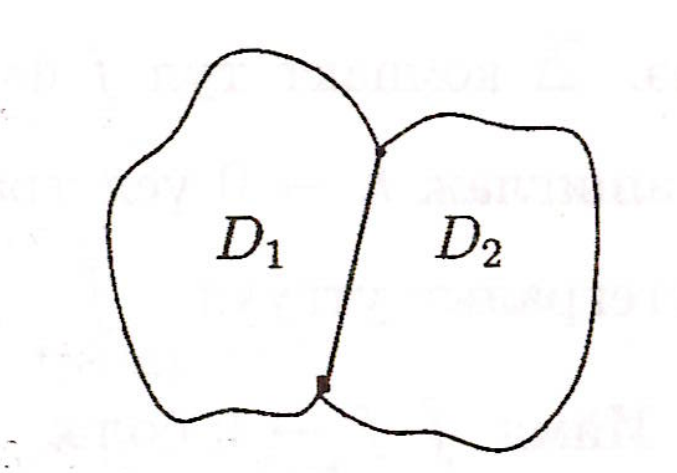
\includegraphics[width=5cm]{Zurag/41.PNG}
    \captionof{figure}{}
        \label{}
\end{center}
$f\in C(D_1\cup \gamma \cup D_2)$ бол $f\in H(D_1\cup \gamma \cup D_2)$ байна. 
\end{lem}
\begin{prf}
Мореры теоремын нөхцөлийг хангасан дурын гурвалжин $\Delta$ авахад $\bint\limits_{\partial \Delta}f(z)dz=0$ гэж харуулбал хангалттай. Уг $\Delta$ нь $\gamma$ хэрчимтэй огтолцоогүй тохиолдолд Кошийн теорем ёсоор $\bint\limits_{\partial \Delta} f=0$ болно.
\begin{center}
    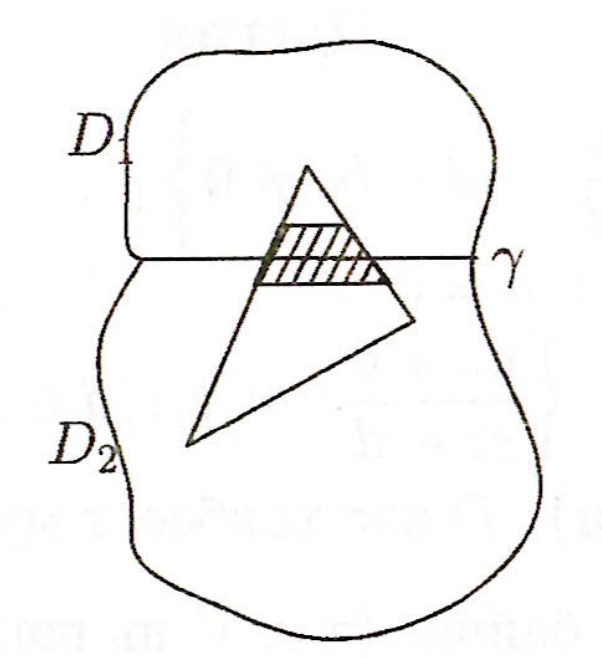
\includegraphics[width=5cm]{Zurag/42.PNG}
    \captionof{figure}{}
        \label{}
\end{center}
Одоо $\Delta$ нь $\gamma$-г зурагт үзүүлсэн байдлаар огтолж байг. $\gamma$-тай параллель түүнээс $h$ зайтай хоёр шулуунаар $T_h$ трапец огтолж авъя. Кошийн теорем ёсоор $\bint\limits_{\partial \Delta} f=\int\limits_{\partial T_h}f$  байна. $h\rightarrow 0$ үед трапецын хажуу ирмэгийн урт тэг рүү тэмүүлэх тул түүгээр авсан интегралын утга багасаж барагдашгүй хэмжигдэхүүн үүсгэнэ. $\overline{\Delta}$ компакт тул $f$ функцийг жигд тасралтгүй болохыг ашиглаж $h\rightarrow 0$ үед трапецын дээд доод ирмэгээр авсан интегралын утгууд $\bint\limits_{(\Delta \cup \gamma)^+}f$ утгыг эсрэг тэмдэгтэйгээр дөхнө. Иймд $\bint\limits_{\partial T_h}f \xrightarrow[h\rightarrow 0]{} 0$ болж  $\bint\limits_{\partial \Delta}f=0$ батлагдав. \\
Харин $\overline{\Delta}$ нь $\gamma$-тай ирмэг ба оройгоор огтолцох тохиолдолд леммын баталгааг дасгал болгон үлдээв. 
\hfill $\blacksquare$\end{prf} 
\begin{thm}
$D_1$ ба $E_1$ нь дээд хагас хавтгайд орших мужууд ба $\gamma\subset \partial D_1$, $\Gamma\subset \partial E_1$ нь бодит тэнхлэгийн хэрчмүүд байг.$D_1$
ба $E_2$ нь $D_1$ ба $E_1$-ийн бодит тэнхлэгийн хувьд тэгш хэмтэй мужууд гэе. $f\in H(D_1)\cap C(D_1\cup \gamma)$ функцийн хувьд $D_1$ мужийг $E_1$ мужид конформ буулгадаг ба $\Gamma =f(\gamma)$ байг. Тэгвэл
$$
\tilde{f}(z)=\begin{cases}
 f(z), \quad z\in D_1\cup \gamma \\
 \overline{f(\overline{z})}, \quad z\in D_2
\end{cases}
$$
функц $D=D_1\cup \gamma \cup D_2$ мужийг $E=E_1\cup \Gamma \cup E_2$ мужид конформ буулгана.
\end{thm}
\begin{prf}
Уг теоремын баталгааг Морерийн теорем ашиглан хийе. $\Delta$ сонгогдоход дараах тохиолдлууд байна.
\begin{enumerate}
    \item $\Delta \subset D_1$ энэ үед Кошийн теорем ёсоор $\bint\limits_{\partial \Delta}\tilde{f}=0$ байна.
    \item $\Delta \subset D_2$ энэ үед уг гурвалжны дээд хагас хавтгай дахь тэгш хэмийг $\Delta_1$ гэвэл
    $$\int\limits_{\partial \Delta^+} \tilde{f}(z)dz=\int\limits_{\partial \Delta^+} \overline{f(\overline{z})}dz=\int\limits_{\partial \Delta^-} \overline{f(z)}d\overline{z}=\overline{\int\limits_{\partial \Delta_1^-} f(z) dz}=\overline{0}=0 $$
    болж батлагдана.
    \item $\Delta \cap \gamma \neq \emptyset$ тохиолдлыг дасгал болгон үлдээв.
\end{enumerate}
\hfill $\blacksquare$\end{prf}
\begin{thm}
 (Риман-Шварцын тэгш хэмийн зарчим). Дээрх теоремын нөхцөлийг $\gamma$ ба $\Gamma$ нь дурын байрлалтай хэрчим эсвэл тойргийн нум болгон өөрчлөн томьёолж болно. Үүнийг Риман- Шварцийн тэгш хэмийн зарчим \index{Риман- Шварцийн тэгш хэмийн зарчим} гэнэ. Энэ ерөнхий тохиолдол нь өмнөх тухайн тохиолдол руу бутархай шугаман буулгалтаар шилждэг.
\end{thm}
\section{Эллипслэг функц}
\begin{dfn}
Коллинеар биш 2 үетэй мероморф функцийг эллипслэг функц гэж тодорхойлдог. Өөрөөр хэлбэл $w=f(z)$ мероморф функц ба $T_1, T_2\in\mathbb{C}\setminus \{0\}:\dfrac{T_1}{T_2}\notin \mathbb{R}$ үед $\forall z:f(z+T_1)=f(z+T_2)=f(z)$  бол уг функцийг эллипслэг функц гэж нэрлэдэг. Дараах жишээг авч үзье. 
$$F(z,k)=\int\limits_{0}^z\frac{dz}{\sqrt{(1-z^2)(1-k^2z^2)}}$$ (энд $0<k<1$ ба $x>0$ үед $\sqrt{x}>0$ мөчир авна). 

Уг функц $\{\im z>0\}$ мужийг
 \begin{align*} \left\{ \right.
    \pm K; \pm K+iK':&K=\int\limits_0^1\frac{dx}{\sqrt{(1-x^2)(1-k^2x^2)}} , \\
    &\left.K'=\int\limits_1^{\frac{1}{k}}\frac{dx}{\sqrt{(x^2-1)(1-k^2x^2)}} \right\}
\end{align*} 
\end{dfn} оройнууд бүхий тэгш өнцөгтөд буулгана. 

Үүний урвуу функцийг авч үзвэл Риман-Шварцийн тэгш хэмийн зарчмаар аналитик үргэлжлэл зохиогдсоор $\mathbb{C}$-д мероморф, эллипслэг функц үүсэх ба үүнийг $w=sn (z,k)$ гээд эллипслэг синус гэж тэмдэглэдэг.
\begin{center}
   \textbf{ Дасгал}
\end{center}
\begin{enumerate}
    \item [4.] Рушегийн теорем ашиглан тэгшитгэлүүд $|z|<1$ дугуйд хэчнээн шийдтэй болохыг тогтоо.
    \begin{enumerate}
        \item [a)] $z^9-2z^6+z^2-8z-2=0;$
        \item [б)] $2z^5-z^3+3z^2-z+8=0;$
        \item [в)] $z^7-5z^4+z^2-2=0$
    \end{enumerate}
    \item [5.] Аргументийн зарчим ашиглан доорх тэгшитгэлүүд баруун хагас хавтгайд $(\re z>0)$ хэдэн шийдтэйг тогтоо.
    \begin{enumerate}
        \item [a)] $z^6+z^5+6z^4+5z^3+8z^2+4z+1=0;$
        \item [б)] $z^4+2z^3+3z^2+z+2=0$
    \end{enumerate}
    \item [6.] $z=0$ цэгийн орчинд голоморф ба $f\left(\dfrac{1}{n}\right)$ дараах дараалал үүсгэдэг функц орших уу?
    \begin{enumerate}
        \item [a)] $0,1,0,1,0,1,\ldots ;$
        \item [б)] $0,\dfrac{1}{2},0, \dfrac{1}{4},0,\dfrac{1}{6}, \ldots ,$
        \item [в)] $\dfrac{1}{2},\dfrac{1}{2},\dfrac{1}{4}, \dfrac{1}{4},\dfrac{1}{6},\dfrac{1}{6}, \ldots ,$
    \end{enumerate}
    \item [7.] $f\in H(D)$ ба $f\neq const$, $f(z)\neq 0 (\forall z\in D)$ бол $|f(z)|$ хамгийн бага утгаа авч чадахгүйг харуул.
    \item [8.] $F(z,k)$ функц $\{\im z>0\}$ мужийг заагдсан тэгш өнцөгтөд буулгадгийг батал.
\end{enumerate}